% University of Michigan Dissertation LaTeX Template for 2019 -- 2020
% Created by John Meluso and Shreyas Kousik
% 9 Jul 2020

% Use the University of Michigan thesis class.
\documentclass[thesis]{thesis-umich}
%%% Packages included in thesis-umich class
%\RequirePackage[margin=1in,footskip=8pt,headsep=0.4cm,headheight=\baselineskip]{geometry}
%\RequirePackage{amsmath}
%\RequirePackage{amsfonts}
%\RequirePackage{amssymb}
%\RequirePackage{graphicx}
%\RequirePackage{subcaption}
%\RequirePackage{times}
%\RequirePackage{natbib}
%\RequirePackage{verbatim}
%\RequirePackage{upquote}
%\RequirePackage{textcomp}
%\RequirePackage{setspace}
%\RequirePackage{ifthen}
%\RequirePackage{soul}
%\RequirePackage{float}
%\RequirePackage[printonlyused]{acronym}
%\RequirePackage{makeidx}
%\RequirePackage{fancyhdr}
%\RequirePackage{multicol}

% Include your packages here by including a \usepackage{<package_name>} command.
\usepackage{blindtext} % Example package which populates the ever-popular lorem ipsum text.

% If you are using the alpha bibliography style, keep these next three lines in your preamble, so that the references are left-aligned; or, you can comment it out and see what happens
\makeatletter
\renewcommand{\@biblabel}[1]{[#1]\hfill}
\makeatother

% Title of the thesis
\title{Your Dissertation Title}

% Author name
\author{Your M. Name}

% Department
\department{Department of You}

% Year of completion
\year=2020

% Author email
\email{youremail@umich.edu}

% Author ORCID iD
\orcid{0000-0000-0000-0000}

% Frontispiece
\frontispiece{
\includegraphics[width=4in]{front_materials/frontispiece.png}}

% Default style for front pages
\frontpagestyle{1} % 7 is preferred by Rackham, but should be set individually for each front page

% Dedication (the input [7] determines the style -- 7 is Rackham's preferred style)
% \hidededication{%
\dedication[7]{
    Put your dedication text here.
}

% Acknowledgments (the input [7] determines the style -- 7 is Rackham's preferred style)
\acknowledgments[7]{ %
    Put your acknowledgements text here.
}
% This command sets the width of the acknowledgments area as a fraction
% of the total width of the text area.
\acknowledgmentswidth{0.8}

% Preface
\hidepreface
%\preface[7]{ %
% Put text here}

% Committee
\committee{ %
Professor First Name, Chair \\
Professor Second Name in Alphabetical Order \\
Professor Third Name in Alphabetical Order \\
Professor Fourth Name in Alphabetical Order
}

% Chair must be entered separately for formatting reasons.
\chair{Professor First Name}
%\cochair{Co-chair One \& Co-chair Two}

% Commands to hide or show lists of figures, tables, etc.
%\hidelistoftables
%\showlistofprograms
%\showlistofappendices


% Definition of any acronyms used.
%\acronyms{}

% Some abstract text
\abstract{
Put your abstract text here.
}
%\hideabstractpagenumber

%% DOCUMENT AREA
\begin{document}

\chapter{Introduction}

This is a dissertation template.
Here is the introduction text.

\section{Example Test}

This dissertation template is motivated by the lack of any others at the time of writing \cite{jefferson2019policing}.
We sincerely hope you find it useful \cite{shannon1948mathematical}.
\section{Example Tables}

You can make a table as follows \cite{ong1997gilbert}.

\begin{table}[ht]
\begin{tabular}{l|l}
\textbf{left column} & \textbf{right column} \\ \hline
entry1 & entry2 \\
entry3 & entry4
\end{tabular}
\caption{An example table with things in it}
\label{tab:my-table}
\end{table}
\section{Example Figure}

Check out Figure \ref{fig:the_big_house}.

\begin{figure}
    \centering
    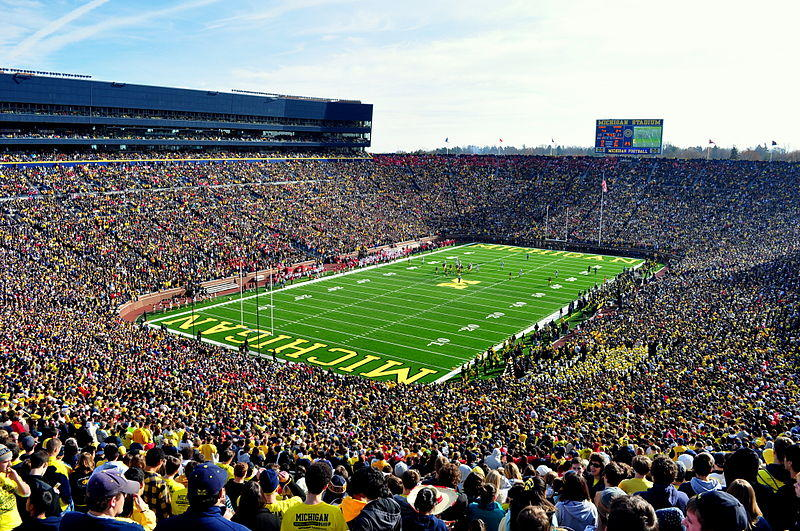
\includegraphics{example_chapter/figures/the_big_house.jpeg}
    \caption{The Big House, taken from Michigan Radio's article about it \cite{the_big_house}}
    \label{fig:the_big_house}
\end{figure}
% Place your additional chapters here using the \input{} command

% Appendices
%\appendix
%\chapter{Methods}
%\chapter{Other Stuff}

\bibliographystyle{alpha}

% Give this command the relative path to the .bib file.
\bibliography{references.bib}

\end{document}
